% tab_benchmarks

\begin{table*}[!t]
\caption{
Benchmark Results
}
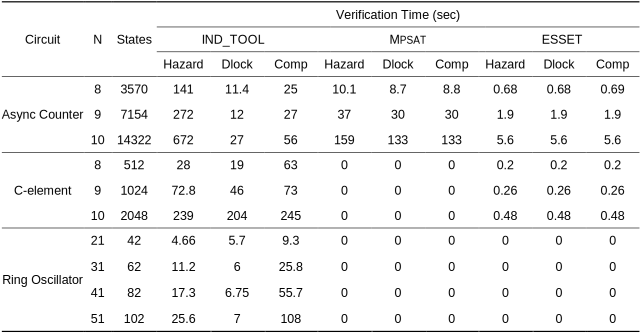
\includegraphics[width=18cm]{figures/tab_benchmarks}
\label{tab_benchmarks}
\end{table*}


\section{Discussion}

\vspace{0.2cm}

\subsection{Performance}

The proposed approach provides a workaround solution to verify asynchronous
circuits using tools that were not built for this purpose. It is therefore
expected that verification performance will be lower compared to dedicated
asynchronous verification tools. In this section we attempt to answer two
questions: (1)~what is the magnitude of performance loss? and (2)~what can we
still verify in feasible time?

One difficulty with answering these questions is that the four verification
tools available to us (that were used in this work) use different verification
approaches that perform better with different types of circuits. For example,
\mpsat{} uses the unfolding technique \cite{khomenko2003model} which makes it
faster when processing highly-concurrent circuits, at the expense of an
overhead for sequential circuits. These differences confound attempts to
establish the overhead of our approach by comparing performance across tools.
Since performance is likely to depend on circuit type, we have selected three
types of benchmark circuits with different scaling characteristics for our
comparison:

\vspace{0.2cm}

\begin{enumerate}
\item $N$-bit counters ($O(N)$ signals, $O(2^N)$ states, fully
sequential),
\item $N$-way C-elements ($O(N)$ signals, $O(2^N)$ states, fully
concurrent), and
\item $N$-stage ring oscillators ($O(N)$ signals, $O(N)$
states, fully sequential).
\end{enumerate}

\vspace{0.2cm}

\Cref{tab_benchmarks} compares verification times for three of the tools we
used (we excluded Xprova from benchmarking since it cannot verify designs with
more than 64 state bits). Based on these results, our conclusions are as
follows. First, for circuits with low degrees of concurrency (e.g. async
counters), \ind{} (with the proposed conversion) has comparable/faster
performance compared to \mpsat{} in deadlock and compliance checks, likely
because \mpsat{} is constructing unfoldings for these purely sequential
circuits. Verification time is still larger for output persistency checks, and
larger in general when comparing with ESSET (which relies on explicit state
space enumeration). Second, for circuits with high degrees of concurrency,
\mpsat{} performs much better than \ind{} (<~0.1 second vs. up to 239
seconds). ESSET performs much better too (< 1 second), although still
noticeably lower than \mpsat{}. Third, \ind{} performs poorly when the number
of circuit components/signals is large, even though when there are few states.
In ring oscillator benchmarks, verification time was 5.7+ seconds for circuits
with as few as 42 states. This is likely because \ind{} explores all possible
values of a~considerably large \texttt{en} vector, as opposed to \mpsat{} and
ESSET which maintain internal lists of enabled transitions and do not have to
re-compute them on each cycle.

In general, benchmark results indicate that there is a considerable
performance overhead when using synchronous tools to verify highly concurrent
asynchronous circuits, compared to asynchronous tools. Even though
asynchronous circuits are often highly concurrent, many mixed systems
consisting of relatively small-sized asynchronous circuits are still well
within the scope of what can be feasibly verified using synchronous tools and
the proposed approach. For example, the mixed system discussed in
\Cref{subsec:mixed} was verified by \ind{} in less than a minute, despite
containing several sync modules (in addition to the async arbiter). We
observed similar results from verifying similar systems
\cite{sokolov2015design} where the number and size of asynchronous handshake
circuits and pipeline controllers was relatively small. For such systems, we
argue that the increase in verification time is offset by the advantage of
being able to verify asynchronous circuits \emph{in-situ}.


% However, given that our synthetic benchmarks are edge
% cases in the design space (i.e. fully concurrent or fully sequential
% circuits), this leaves the question of how synchronous tools fair on realistic
% designs consisting of both sync and async parts. While it is still difficult
% to answer this question generally, the reported benchmarks


% the performance of Incisive
% Formal and MPSat using cascades of the asynchronous handshaking element shown
% in Figure~??, as a rough estimation of performance differences. We chose this
% circuit because it has no concurrency that can be exploited by MPSat's
% unfolding technique, making it a good candidate for a direct comparison. The
% results are shown in Figure~X, for 8, 9 and 10 stage cascades.

% So, we have three potential sets of scalable and simple benchmarks: 1) N-bit
% counter: O(N) signals, O(2^N) states, fully sequential, 2) N-way C-element:
% O(N) signals, O(2^N) states, fully concurrent, 3) N-stage repeater (N
% connected buffers): O(N) signals, O(N) states, fully sequential. Logically
% this seems to cover all interesting combinations. 1+2 show how performance
% scales wrt to concurrency in the system. 3 highlights the scaling of tools wrt
% the number of signals (where the exponential explosion in states does not
% dominate the complexity). It may be worth including all of these.


\subsection{Related Work}
\label{subsec:related}

Our approach is inspired by prior research by the asynchronous circuits
community, in particular:

\begin{itemize}

\item Roncken et al.~\cite{roncken2015naturalized} use \texttt{go} signals to
control progress in asynchonrous circuits in a fine-grained manner for the
purpose of silicon test and debug. The idea is further developed
in~\cite{chau2017framework}, where \texttt{go} signals are used to model
non-determinism in asynchonrous circuits in the context of formal verification
of \emph{link-joint} models using the theorem proving system ACL2.

\item Dobkin et al.~\cite{dobkin2008assertion} present an algorithm for
converting STGs into sets of assertions written in the Property Specification
Language (PSL), which can be used by standard assertion-based verification
tools for synchronous designs. This approach allows the designer to verify the
correct behaviour of synchronous circuits against a model of the asynchonrous
part of the system.

\end{itemize}

In general, the idea of clocking an asynchonrous circuit is not new.
\cite{peeters2001synchronous} presents a synchronous back-end for the Tangram
compiler with two aims: (i) providing a fast approach for prototyping asynchronous
circuits using synchronous FPGAs, and (ii) reducing the risk of adoption of
asynchonrous design methodology in industry by supporting the synchronous mode of
execution as a fall-back scenario. \cite{van2003adding} introduced a systematic
approach for testing and debugging of asynchonrous circuits by incorporating
conventional synchronous scan-chains. Elastic circuits~\cite{carmona2009elastic}
provide a way to achieve many of the benefits of asynchonrous circuits through
conventional synchronous design flow. This paper follows this direction of
research but in the context of formal verification.

% There are many approaches and tools developed for model-based verification of
% asynchonrous circuits. We only mention three of them due to the lack of space:
% 1) STGs are supported by an efficient verification backend integrated in
% open-source framework Workcraft~\cite{poliakov2008automated}; 2) an
% ACL2-powered method for verification of high-level asynchronous networks
% described using \emph{click} primitives is presented
% in~\cite{verbeek2013formal}; 3) a tool for formal verificatrion of GALS
% networks described using xMAS communication primitives is presented
% in~\cite{burns2017structured}.

There are existing industrial design flows relying on conventional EDA tools
for mixed sync-async systems. For example, \cite{yakovlev2013advances}
describes the design flow developed by Tiempo, but without providing
implementation details of the underlying formal verification methodology.
Proteus~\cite{beerel2011proteus} is another example of an industrial design
flow developed by TimeLess Design Automation, which uses CSP as the
specification language~\cite{beerel2010designer}. As described
in~\cite{beerel2011proteus}, Proteus has no support for formal verification of
async circuits, but uses cosimulation and proprietary coverage tools to ensure
that an implementation-environment pair matches the CSP specification.
